\section{Von der Recherche zum Feinkonzept}
Um Eckpfeiler für die zu Beginn des Projekts benötigten Recherchen zu erhalten, musste das Problem grob in seine Einzelteile zerlegt werden. Aus dieser Zerlegung resultierten die Bereiche Kommunikation zwischen elektronischen Geräten, Möglichkeiten zur Objekterkennung und Objektverfolgung, diverse Flugobjekte und Fahrantriebe, Bedarf von Dreh- und Wurfmechanismen sowie das Versorgungskonzept. 
Nach der Recherche folgte als nächster Schritt das Erstellen einer Funktionsskizze, um daraus die einzelnen Teilprobleme zu eruieren.
\begin{figure}[h!]
	\centering
	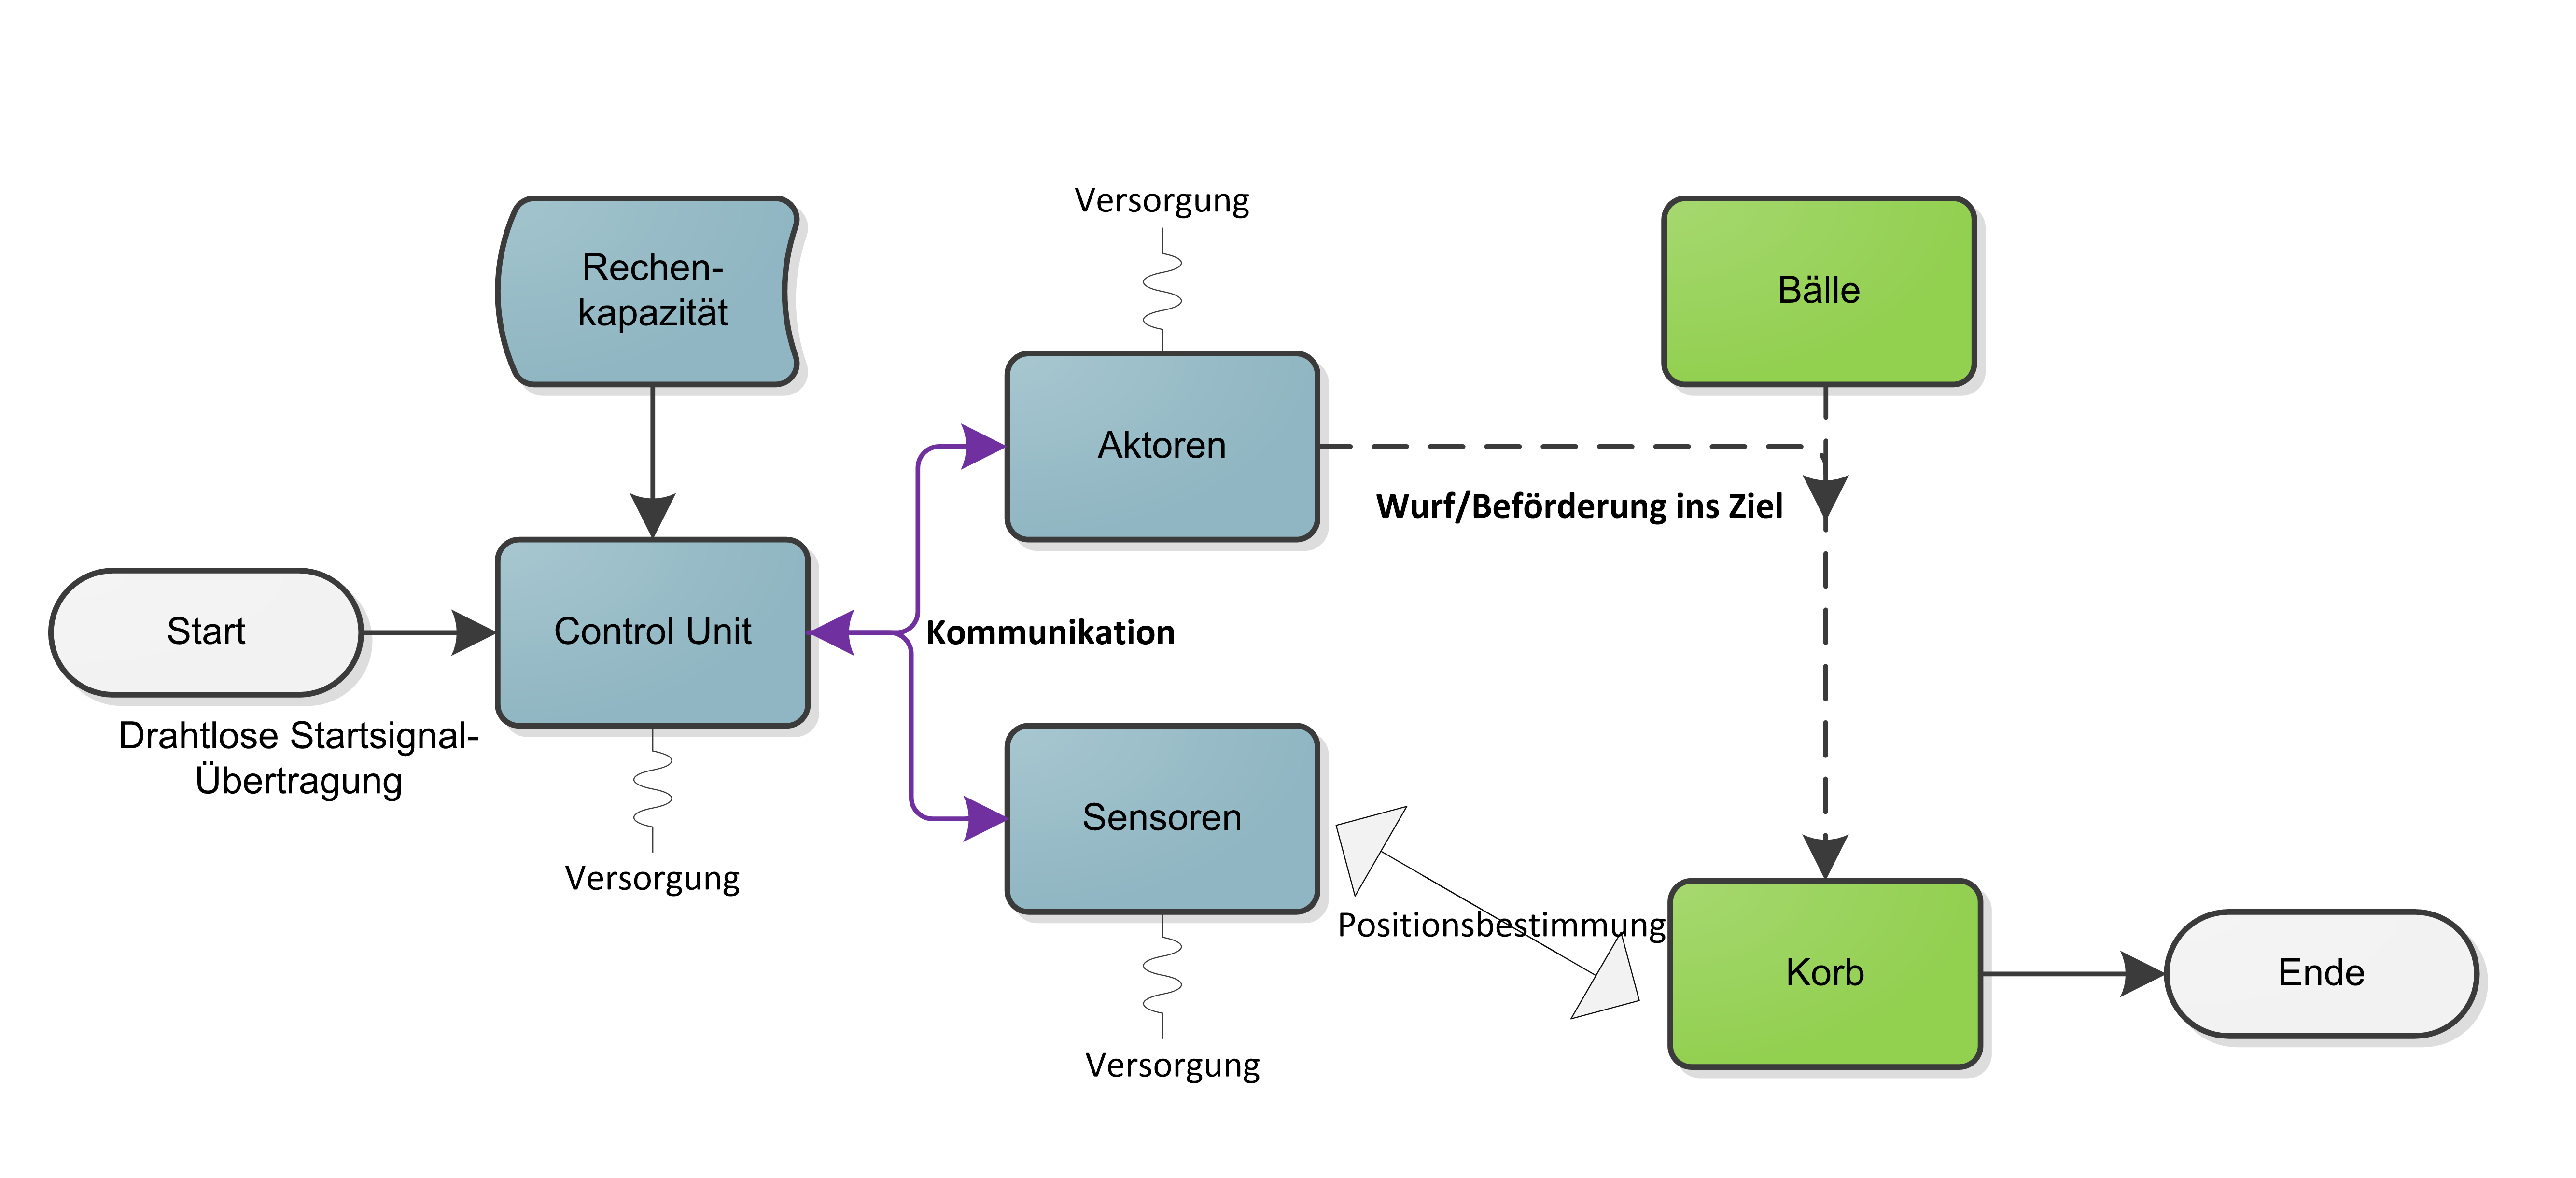
\includegraphics[width=0.9\textwidth]{Enddokumentation/Varianten/Bilder/Funktionsskizze.png}
	\caption{Funktionsskizze}
	\label{fig:Funktionsskizze}
\end{figure}
Nach der Ermittlung dieser Teilprobleme mussten für die einzelnen Bereiche nach Lösungsansätzen recherchiert werden. Die Resultate dieser Recherche, sowie die danach folgende Bewertung der gefundenen Lösungen ist aus Platzgründen im Anhang hinterlegt. Um die Ergebnisse der Bewertung sinnvoll als Entscheidungshilfe einsetzen zu können, wurden sie kompakt zu einem Grobkonzept zusammengefasst.\\
\\
\begin{figure}
	\centering
	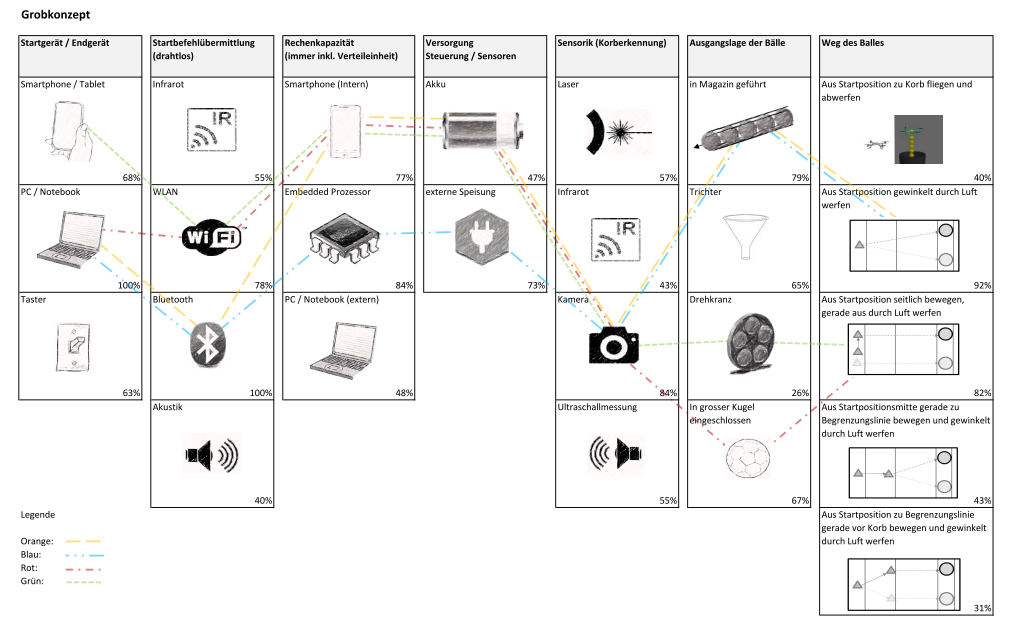
\includegraphics[width=0.9\textwidth]{Enddokumentation/Varianten/Bilder/Grobkonzept.png}
	\caption{Grobkonzept}
	\label{fig:Grobkonzept}
\end{figure}
Das Grobkonzept erlaubt es grafisch verschiedene Kombinationsmöglichkeiten aufzuzeigen. Um möglichst vielen differenzierten Ansätzen Rechnung zu tragen, wurden vier Varianten während einer Diskussionsrunde festgelegt.\\\\ 
!!!!! Achtung: wenn Grobkonzept mit Bild im Text, Variantennummern in Farben umbenennen. !!!!\\\\
Eine Variante ist die Kombination aller Lösungsansätze mit der höchsten Prozentzahl. Eine zweite Variante basiert auf der Idee, die Bälle in eine Kugel einzuschliessen, das Gerät parallel zur Spielfeldwand zu verschieben und den Korb mit einer Smartphone-Kamera zu erkennen. Der Ballwerfer soll durch einen Akkumulator mit Energie versorgt werde. Die dritte Variante hat als Ausgangspunkt die Bälle in einem Drehkranz und befördert diese einzeln in den Korb, die restlichen Kriterien werden Kongruent zur zweiten Variante ausgeführt. In der vierten Variante befördert der Ballwerfer die Bälle aus der Startposition in bogenförmiger Kurve in den Korb. Die Ausgabe der Bälle erfolgt vereinzelt, die übrigen Teilprobleme verwenden wiederum, kongruent zur zweiten Variante eine Smartphone-Kamera zur Korberkennung und ein Akkumulator als Energieversorgung.\\
\\
Die Entscheidung fiel auf die vierte Variante. Diese bietet als gesamtes Konzept die erfolgversprechendste und effizienteste Lösung, bezüglich der Zielsetzung des Teams. // Verweis definierte Ziele.\\
\\
Nach der Entscheidung für eine Variante folgt die weitere Ausarbeitung dieses Konzeptes
in ein Feinkonzept. Die ursprünglich sieben Teilprobleme wurden in 19 Subteilprobleme
aufgesplittet. Zu jedem Subteilproblemen existieren wiederum Lösungsvarianten. Im Unterschied zum Grobkonzept erfolgt die Bewertung nicht mit Prozenten, sondern werden die Lösungsvarianten miteinander verglichen und nach aktuellem Wissenstand eine oder eventuell auch mehrere Lösungsvarianten ausgewählt. 


